% This file was created by matplotlib2tikz v0.6.18.
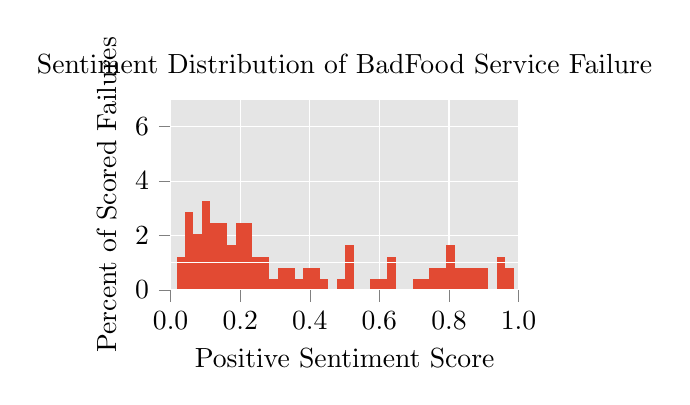
\begin{tikzpicture}

\definecolor{color0}{rgb}{0.886274509803922,0.290196078431373,0.2}

\begin{axis}[
axis background/.style={fill=white!89.80392156862746!black},
axis line style={white},
height=4cm,
tick align=outside,
tick pos=left,
title={Sentiment Distribution of BadFood Service Failure},
width=6cm,
x grid style={white},
xlabel={Positive Sentiment Score},
xmajorgrids,
xmin=0, xmax=1,
xtick={0,0.2,0.4,0.6,0.8,1},
xticklabels={0.0,0.2,0.4,0.6,0.8,1.0},
y grid style={white},
ylabel={Percent of Scored Failures},
ymajorgrids,
ymin=0, ymax=7
]
\draw[fill=color0,draw opacity=0] (axis cs:0.017034936696291,0) rectangle (axis cs:0.0412680432200432,1.22571873114969);
\draw[fill=color0,draw opacity=0] (axis cs:0.0412680432200432,0) rectangle (axis cs:0.0655011534690857,2.86001015285175);
\draw[fill=color0,draw opacity=0] (axis cs:0.0655011534690857,0) rectangle (axis cs:0.0897342637181282,2.04286408085011);
\draw[fill=color0,draw opacity=0] (axis cs:0.0897342562675476,0) rectangle (axis cs:0.11396735906601,3.26858353430113);
\draw[fill=color0,draw opacity=0] (axis cs:0.11396735906601,0) rectangle (axis cs:0.138200461864471,2.45143765072585);
\draw[fill=color0,draw opacity=0] (axis cs:0.138200461864471,0) rectangle (axis cs:0.162433564662933,2.45143765072585);
\draw[fill=color0,draw opacity=0] (axis cs:0.162433564662933,0) rectangle (axis cs:0.186666682362556,1.63429076220991);
\draw[fill=color0,draw opacity=0] (axis cs:0.186666682362556,0) rectangle (axis cs:0.210899785161018,2.45143765072585);
\draw[fill=color0,draw opacity=0] (axis cs:0.210899785161018,0) rectangle (axis cs:0.23513288795948,2.45143765072585);
\draw[fill=color0,draw opacity=0] (axis cs:0.235132902860641,0) rectangle (axis cs:0.259366035461426,1.22571807165744);
\draw[fill=color0,draw opacity=0] (axis cs:0.259366005659103,0) rectangle (axis cs:0.283599108457565,1.22571882536292);
\draw[fill=color0,draw opacity=0] (axis cs:0.283599108457565,0) rectangle (axis cs:0.307832211256027,0.408572941787641);
\draw[fill=color0,draw opacity=0] (axis cs:0.307832211256027,0) rectangle (axis cs:0.332065314054489,0.817145883575282);
\draw[fill=color0,draw opacity=0] (axis cs:0.332065314054489,0) rectangle (axis cs:0.356298416852951,0.817145883575282);
\draw[fill=color0,draw opacity=0] (axis cs:0.356298416852951,0) rectangle (axis cs:0.380531519651413,0.408572941787641);
\draw[fill=color0,draw opacity=0] (axis cs:0.380531519651413,0) rectangle (axis cs:0.404764622449875,0.817145883575282);
\draw[fill=color0,draw opacity=0] (axis cs:0.404764622449875,0) rectangle (axis cs:0.428997725248337,0.817145883575282);
\draw[fill=color0,draw opacity=0] (axis cs:0.428997755050659,0) rectangle (axis cs:0.453230887651443,0.408572439317625);
\draw[fill=color0,draw opacity=0] (axis cs:0.453230857849121,0) rectangle (axis cs:0.477463960647583,0);
\draw[fill=color0,draw opacity=0] (axis cs:0.477463960647583,0) rectangle (axis cs:0.501697063446045,0.408572941787641);
\draw[fill=color0,draw opacity=0] (axis cs:0.501697063446045,0) rectangle (axis cs:0.525930166244507,1.63429176715056);
\draw[fill=color0,draw opacity=0] (axis cs:0.525930166244507,0) rectangle (axis cs:0.550163269042969,0);
\draw[fill=color0,draw opacity=0] (axis cs:0.550163269042969,0) rectangle (axis cs:0.574396371841431,0);
\draw[fill=color0,draw opacity=0] (axis cs:0.574396371841431,0) rectangle (axis cs:0.598629474639893,0.408572941787641);
\draw[fill=color0,draw opacity=0] (axis cs:0.598629474639893,0) rectangle (axis cs:0.622862577438354,0.408572941787641);
\draw[fill=color0,draw opacity=0] (axis cs:0.622862577438354,0) rectangle (axis cs:0.647095680236816,1.22571882536292);
\draw[fill=color0,draw opacity=0] (axis cs:0.647095680236816,0) rectangle (axis cs:0.671328783035278,0);
\draw[fill=color0,draw opacity=0] (axis cs:0.671328783035278,0) rectangle (axis cs:0.69556188583374,0);
\draw[fill=color0,draw opacity=0] (axis cs:0.69556188583374,0) rectangle (axis cs:0.719794988632202,0.408572941787641);
\draw[fill=color0,draw opacity=0] (axis cs:0.719794988632202,0) rectangle (axis cs:0.744028091430664,0.408572941787641);
\draw[fill=color0,draw opacity=0] (axis cs:0.744028091430664,0) rectangle (axis cs:0.768261253833771,0.817143873697689);
\draw[fill=color0,draw opacity=0] (axis cs:0.768261253833771,0) rectangle (axis cs:0.792494356632233,0.817145883575282);
\draw[fill=color0,draw opacity=0] (axis cs:0.792494356632233,0) rectangle (axis cs:0.816727459430695,1.63429176715056);
\draw[fill=color0,draw opacity=0] (axis cs:0.816727459430695,0) rectangle (axis cs:0.840960562229156,0.817145883575282);
\draw[fill=color0,draw opacity=0] (axis cs:0.840960562229156,0) rectangle (axis cs:0.865193665027618,0.817145883575282);
\draw[fill=color0,draw opacity=0] (axis cs:0.865193665027618,0) rectangle (axis cs:0.88942676782608,0.817145883575282);
\draw[fill=color0,draw opacity=0] (axis cs:0.88942676782608,0) rectangle (axis cs:0.913659870624542,0.817145883575282);
\draw[fill=color0,draw opacity=0] (axis cs:0.913659870624542,0) rectangle (axis cs:0.937892973423004,0);
\draw[fill=color0,draw opacity=0] (axis cs:0.937892973423004,0) rectangle (axis cs:0.962126076221466,1.22571882536292);
\draw[fill=color0,draw opacity=0] (axis cs:0.962126076221466,0) rectangle (axis cs:0.986359179019928,0.817145883575282);
\path [draw=white, fill opacity=0] (axis cs:0,0)
--(axis cs:0,7);

\path [draw=white, fill opacity=0] (axis cs:1,0)
--(axis cs:1,7);

\path [draw=white, fill opacity=0] (axis cs:0,0)
--(axis cs:1,0);

\path [draw=white, fill opacity=0] (axis cs:0,1)
--(axis cs:1,1);

\end{axis}

\end{tikzpicture}